\chapter{Flight Data \label{ch:flight_data}}
After having found the set of optimal calibration parameters and applying them to the flight data of \ac{SETH} junior, roll and pitch angles, as well as the gondola's heading or orientation, can be calculated. How this is done has been described in sec.~\ref{sec:meth:determination_heading} on page~\pageref{sec:meth:determination_heading}.

The upper plot in fig.~\ref{fig:res:flight_heading} presents the pitch angle in red and the roll angle in blue, plotted against time. The lower plot presents the gondola's heading against time. The angle of heading is given from 0$^\circ$ to 360$^\circ$ as written on a compass with $0^\circ\equiv\mathrm{North}$, $90^\circ\equiv\mathrm{East}$, etc.\\
It can be seen that the gondola's swinging is strongest after launch and during ascent until it calms down at higher altitudes.\\
The timestamp on the x-axis has been corrected to show the correct time in~UTC. The Raspberry~Pi has an internal clock that is used during flight. If the time is not set manually, it continues counting up from the time when it was last shut off. This resulted in a time difference of 3433\,s that the Pi was lagging behind.

\begin{figure}[H]
    \centering
    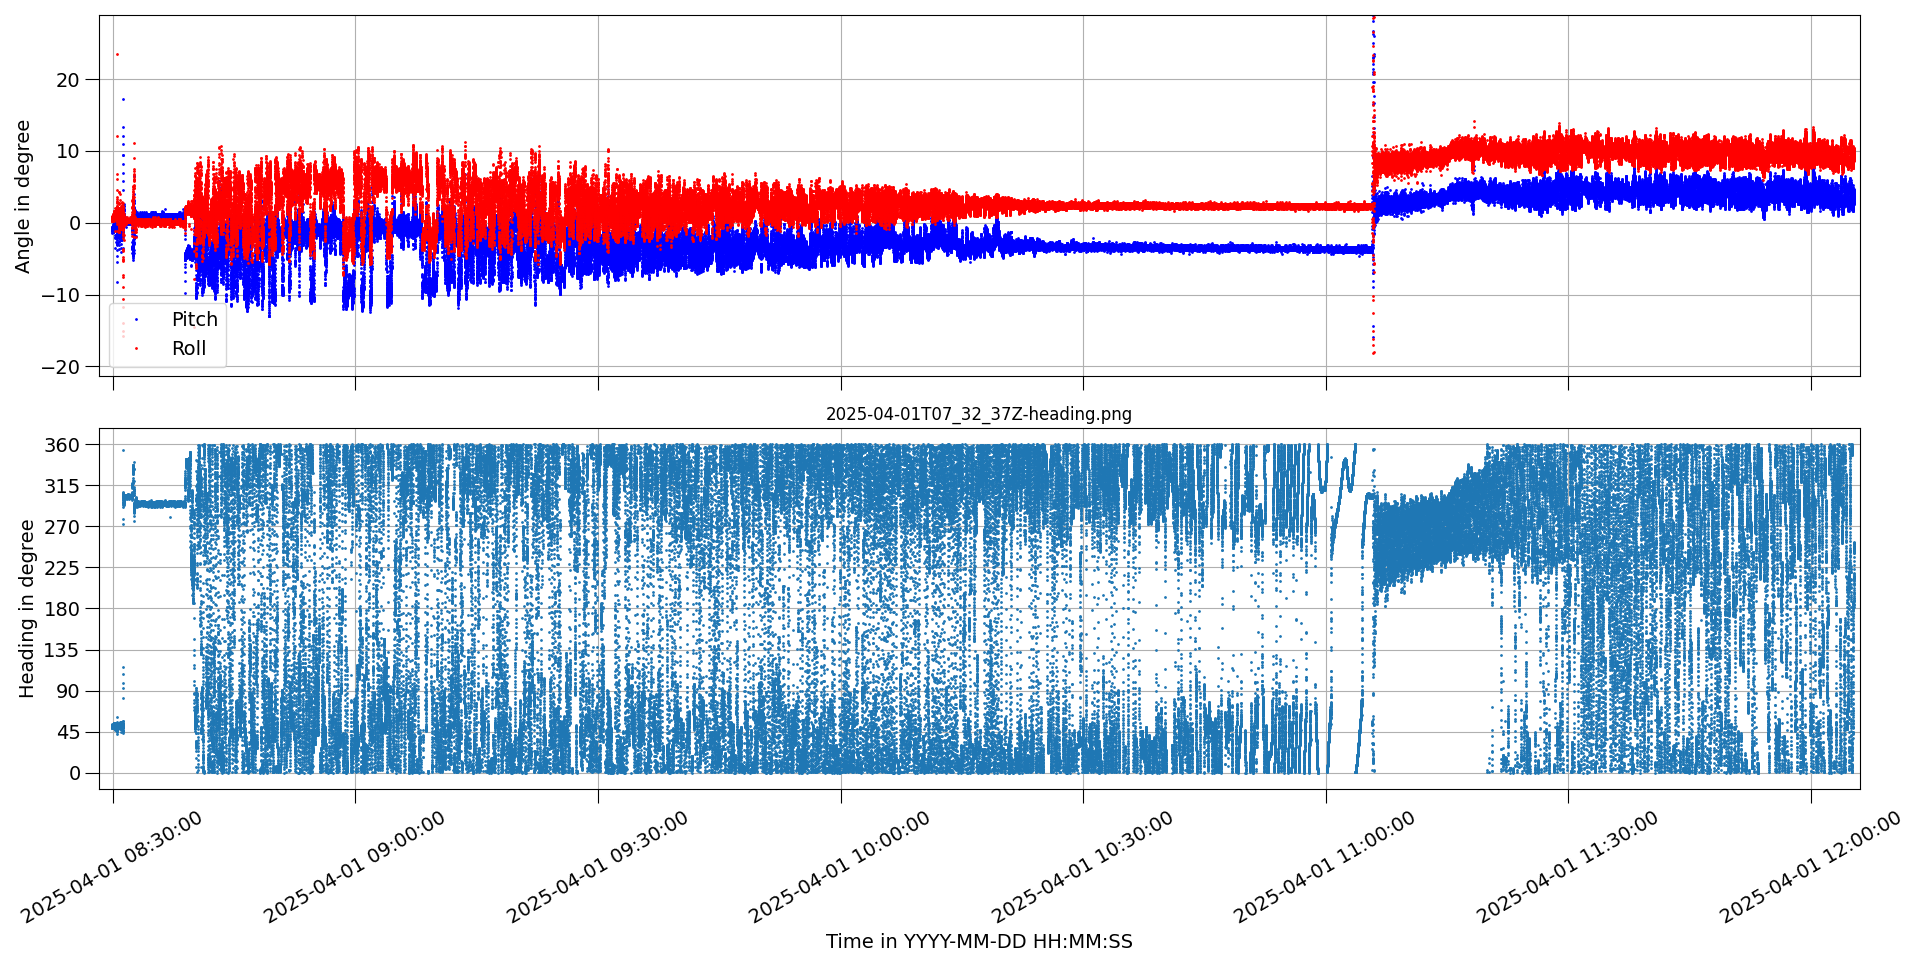
\includegraphics[width=\linewidth]{images/05_flight_data/flight_heading.png}
    \caption{Pitch, roll and heading during the whole flight.}
    \label{fig:res:flight_heading}
\end{figure}

The balloon launch is around 10:40 local time or 8:40~UTC. After this time, the balloon starts its ascent, the gondola swinging and rotating below it. The swinging gradually decreases with time and altitude until it is calmest before the burst of the balloon. The rotational frequency is seemingly constant, but also decreases before the burst. Afterwards the payload's heading rocks around the East-North-East direction and continues swinging. It can be assumed that the parachute does not decelerate the gondola uniformly but pulls it in one direction as the red curve is shifted upwards.

\section{Pre-Launch Phase \label{sec:pre-launch_phase}}
We use photos from the pre-launch phase to confirm that all calculations of pitch, roll and heading are done correctly. The three moments before launch that we show are: The gondola laying on the ground looking in two different directions and the gondola being put down after it was picked up. The camera points in the same direction as the positive x-axis which is equivalent to the heading. Figures~\ref{fig:fd:apeman_50} and~\ref{fig:fd:apeman_300} show the two directions that the camera looks at for longer periods of time before launch. It can be seen that the gondola's headings in the photos are 50\deg and 300\deg respectively, when looking for the corresponding timestamps in fig.~\ref{fig:fd:pre-launch_heading}.

\begin{figure}[h]
\begin{subfigure}[t]{.4999\textwidth}
  \centering
  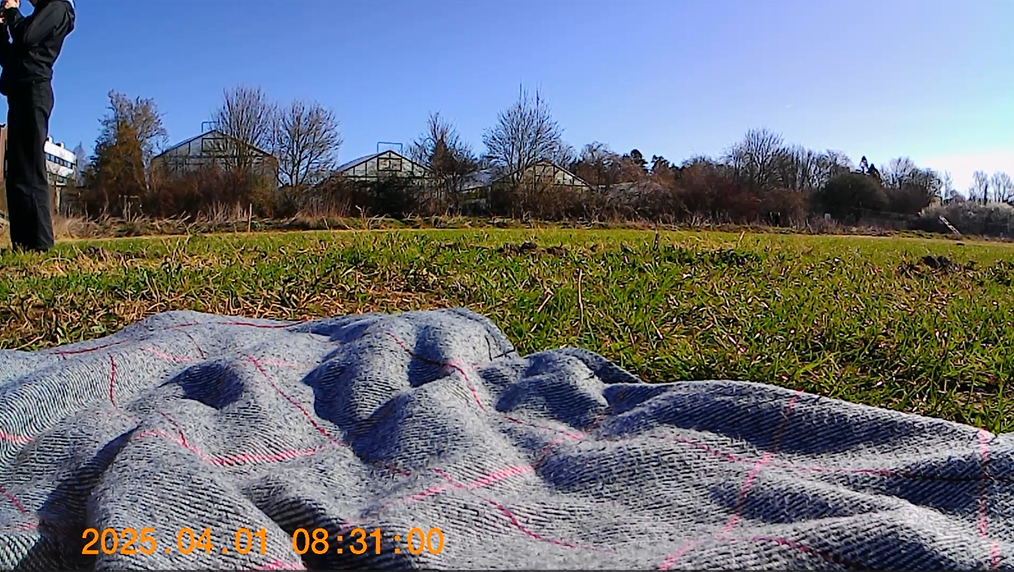
\includegraphics[width=.9\linewidth]{images/05_flight_data/apeman_50_8_31_00.png}
  \caption{Looking at three greenhouses at 8:31:00. The university's biology building can be seen on the left hand side.}
  \label{fig:fd:apeman_50}
\end{subfigure}
\begin{subfigure}[t]{.4999\textwidth}
  \centering
  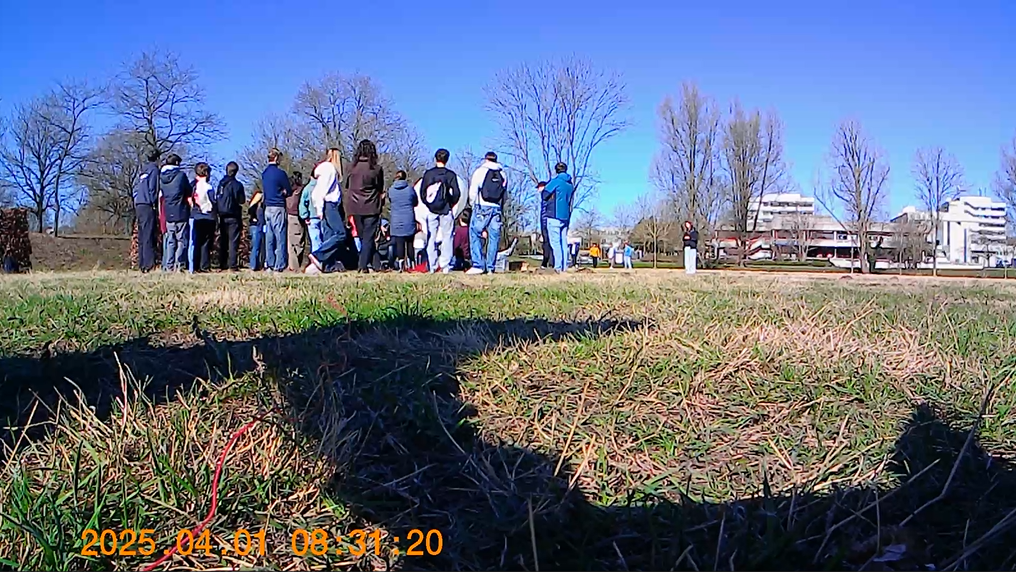
\includegraphics[width=.9\linewidth]{images/05_flight_data/apeman_300_8_31_20.png}
  \caption{Looking at a treeline in front of Mensa II at 8:31:20.}
  \label{fig:fd:apeman_300}
\end{subfigure}
\caption{Photos taken by the camera aboard \ac{SETH} junior.}
\label{fig:fd:apeman_headings}
\end{figure}

\begin{figure}[h]
    \centering
    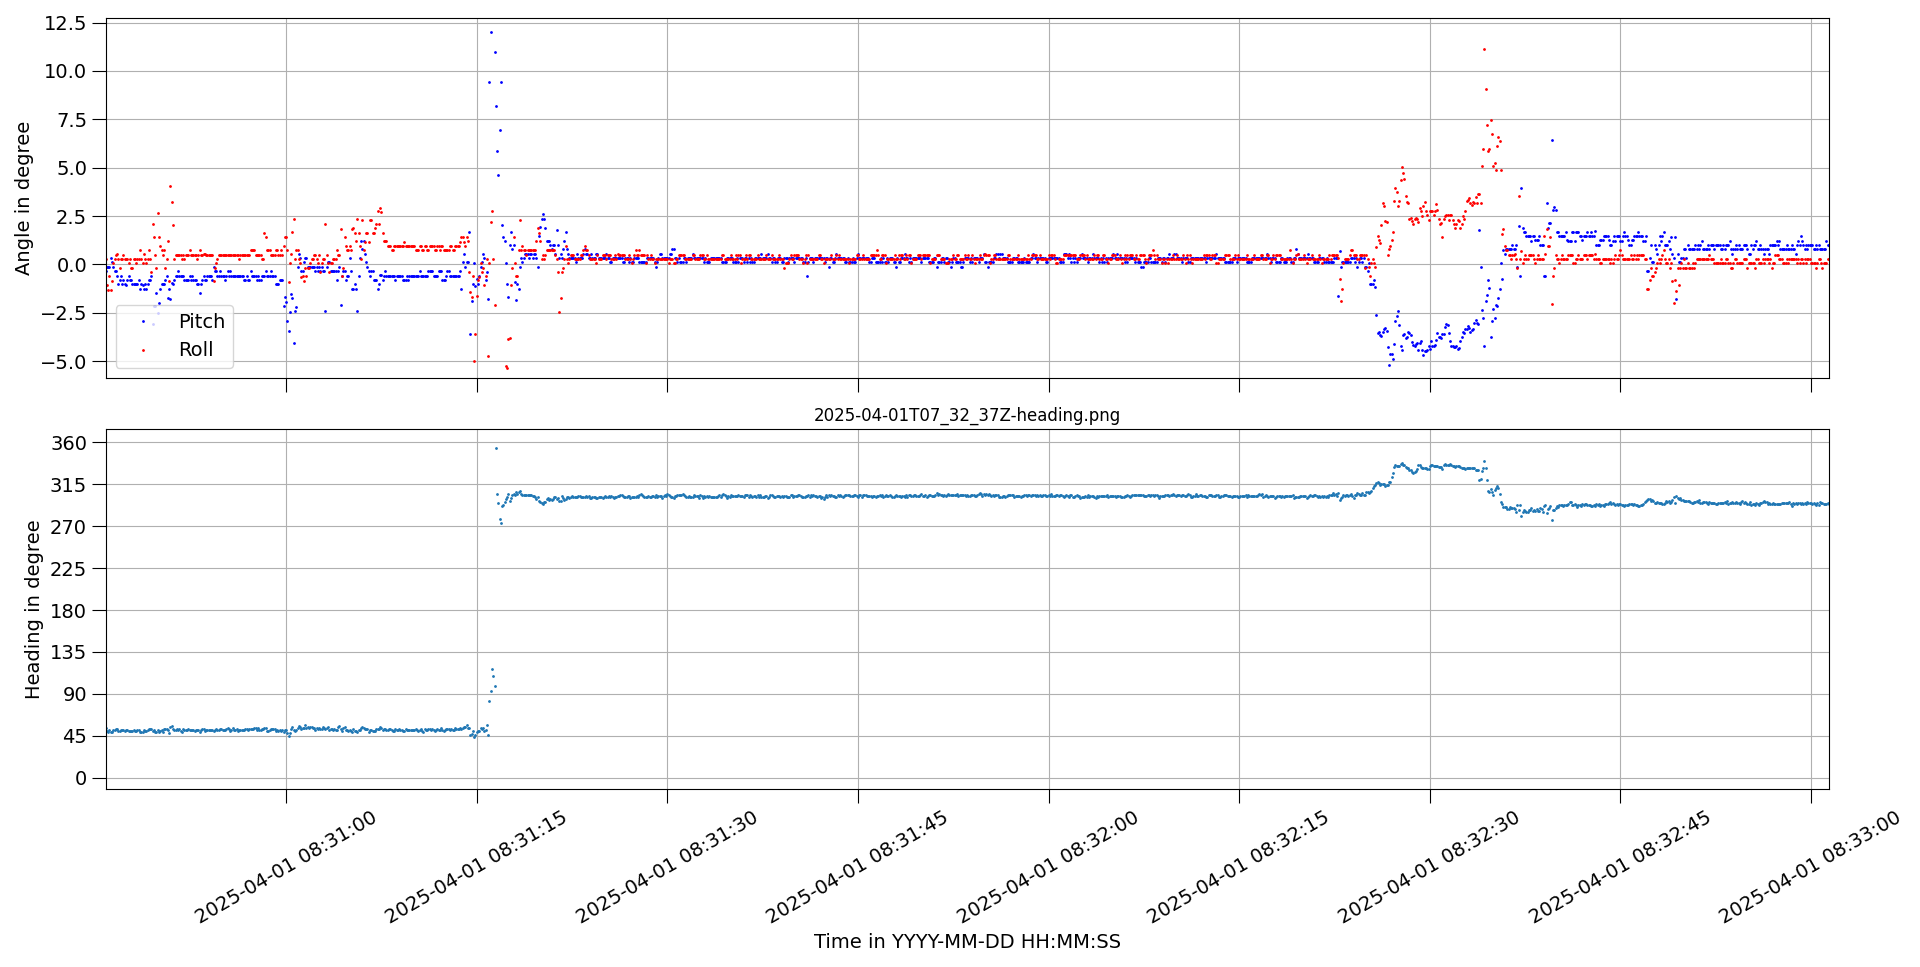
\includegraphics[width=\linewidth]{images/05_flight_data/pre-launch_heading.png}
    \caption{Roll, pitch and heading before the launch.}
    \label{fig:fd:pre-launch_heading}
\end{figure}

Figure~\ref{fig:fd:compass_rose} shows a satellite image of the launch area with a compass rose centred around the approximate location where \ac{SETH} jr. was prepared. The 50\deg and 300\deg angles are marked with red lines. It can be seen that there are the same greenhouses diagonally in front of the biology building as are seen in fig.~\ref{fig:fd:apeman_50}. The same tree seen in the centre of fig.~\ref{fig:fd:apeman_300} can be seen right beneath the 300\deg marking in fig. \ref{fig:fd:compass_rose}. From this we gather that the heading calibration and calculation are done correctly.

\begin{figure}[h]
    \centering
    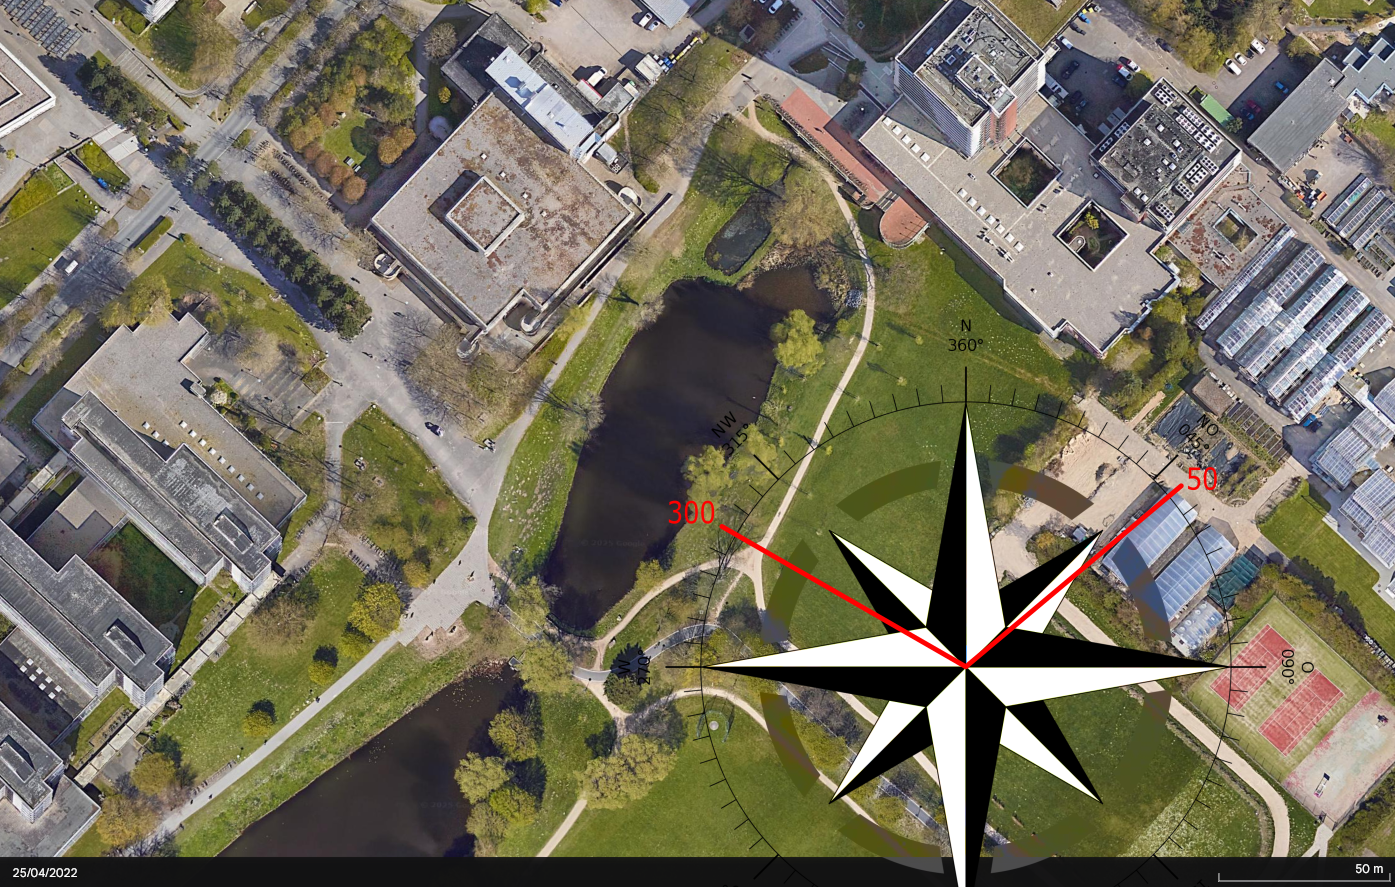
\includegraphics[width=\linewidth]{images/05_flight_data/launch_location_compass.png}
    \caption{Satellite image of the launch area. In the centre of the compass rose is the approximate location where \ac{SETH} jr. was set down while preparing the balloon and flight train. Marked in red are the 300\deg and 50\deg heading.}
    \label{fig:fd:compass_rose}
\end{figure}

Figure~\ref{fig:fd:apeman_roll}, taken at 8:32:35, shows the moment the gondola is being set back down after it was picked up. Marked with two red lines are a horizontal line and a line showing the approximate horizon. The lines are at an angle of 4.7\deg to each other. The coordinate system of the gondola's body frame is shown in the lower centre of the image. Because the camera is looking in the positive x-direction, the roll angle of 4.7\deg is in mathematically positive direction. It can be seen that the gondola experiences a positive roll when comparing with the same time in fig.~\ref{fig:fd:pre-launch_heading}. With this we have shown that the calculation of the roll (and by similarity pitch) angle is done correctly. The $3433\,\mathrm{s}$ time difference of the Raspberry is accepted as correct because when comparing fig.~\ref{fig:fd:pre-launch_heading} with the camera's video, a match of time and events can only be verified within approximately two seconds.

\begin{figure}[h]
    \centering
    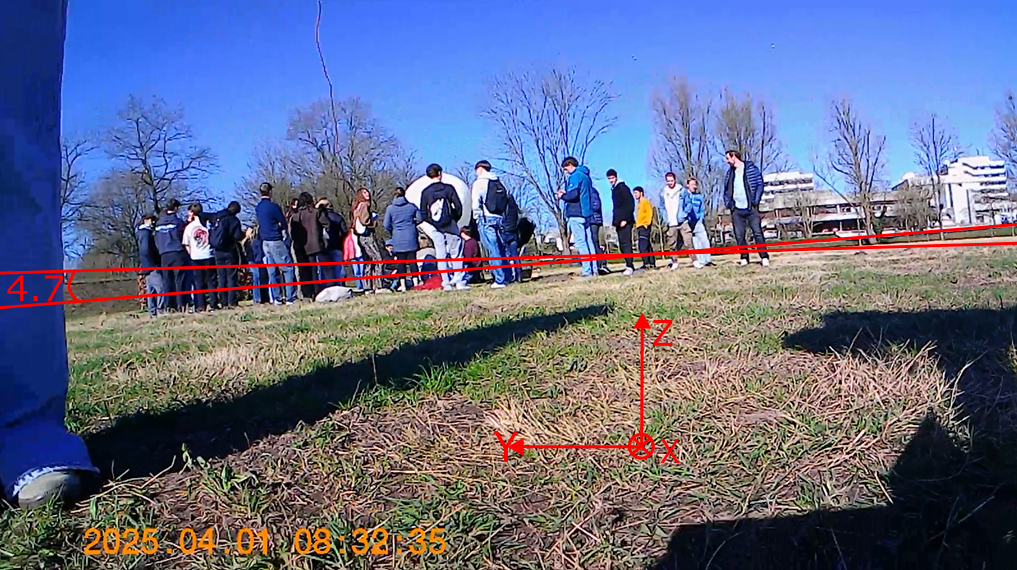
\includegraphics[width=0.8\linewidth]{images/05_flight_data/apeman_roll_8_32_35.png}
    \caption{A photo taken at 8:32:35 showing the ground rotated against the horizontal plane.}
    \label{fig:fd:apeman_roll}
\end{figure}

\section{Launch \label{sec:launch}}
The balloon is launched just before 8:40~UTC as fig.~\ref{fig:res:launch_heading} shows. The figure is held in the same style as described previously.\\
It can be seen that the gondola rotates quickly at about 5 revolutions per minute (rpm). Swinging of the gondola is also strong, with a peak-to-peak amplitude of around 10$^\circ$ in roll and pitch. In the first ten minutes, the roll angle is relatively symmetric around 0\deg while the pitch angle is centred around the -5$^\circ$ mark. This can be explained by a possibly asymmetric suspension.

\begin{figure}[H]
    \centering
    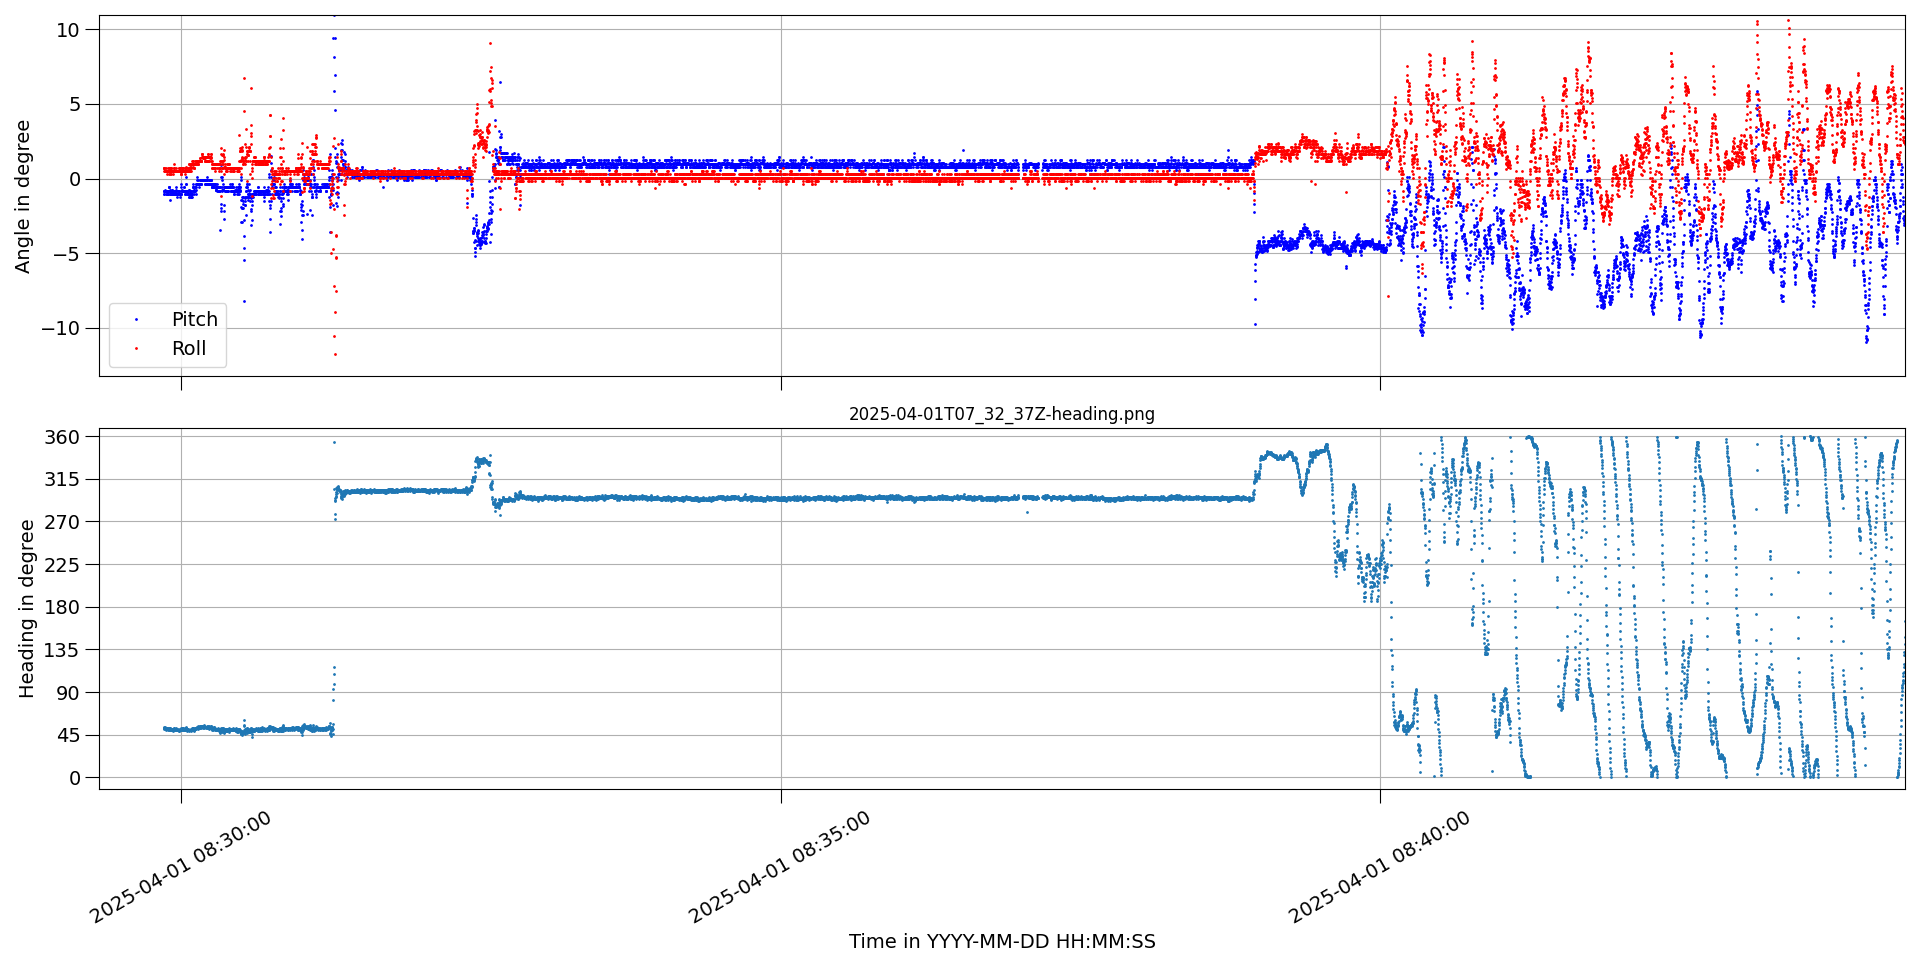
\includegraphics[width=\linewidth]{images/05_flight_data/launch_heading.png}
    \caption[Heading at launch.]{Pitch, roll and heading around launch.}
    \label{fig:res:launch_heading}
\end{figure}


\section{Ascent \label{sec:ascent}}
Figure~\ref{fig:res:ascent_heading} shows that the rotation of the gondola slows down to approximately 4~rpm. The swinging decreases significantly to a peak-to-peak amplitude of 2 to 5 degrees.

\begin{figure}[H]
    \centering
    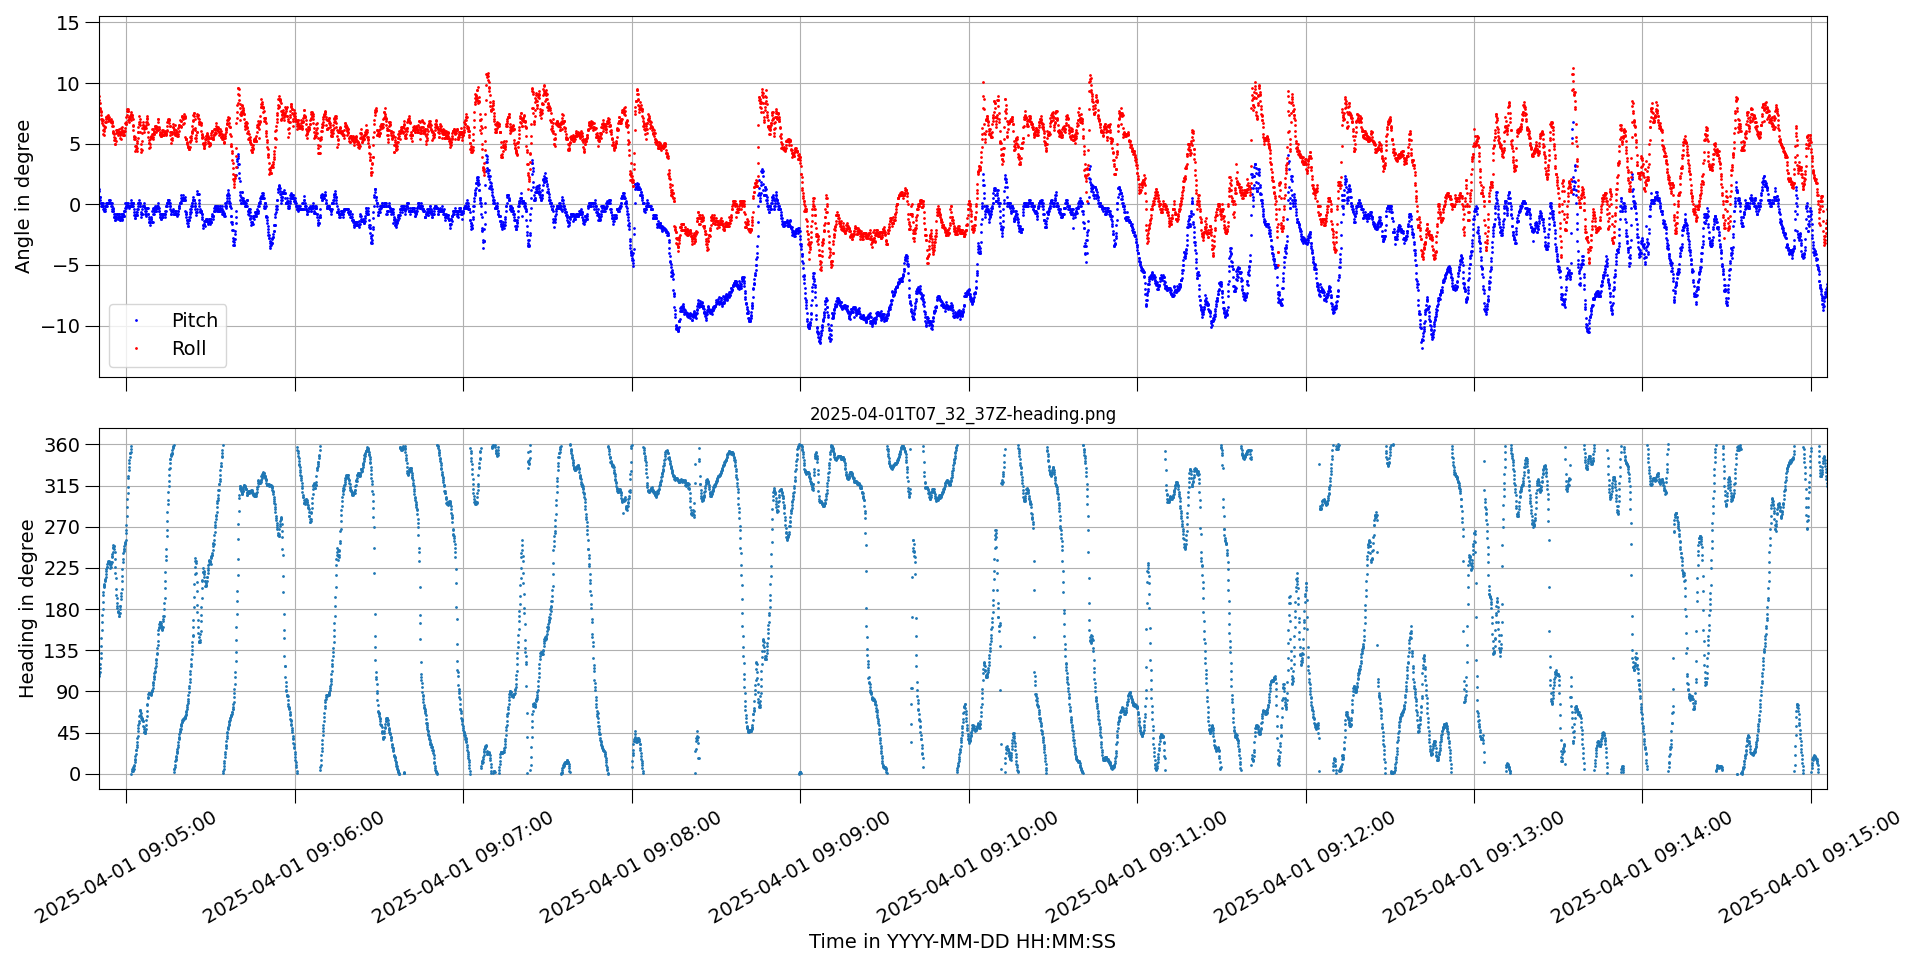
\includegraphics[width=\linewidth]{images/05_flight_data/mid_flight_heading.png}
    \caption[Heading during ascent.]{Pitch, roll and heading during ascent.}
    \label{fig:res:ascent_heading}
\end{figure}


\section{Balloon Burst \label{sec:balloon_burst}}
The balloon burst at approximately 11:06~UTC as fig.~\ref{fig:res:burst_heading} shows. It can also be seen in the upper plot that the roll and pitch angles are constantly different from zero. In addition to the previously discussed asymmetric suspension the payload may have a non-uniform weight distribution. Until now it was assumed that the centre of mass would be somewhere on the box's vertical axis. If that is not the case, the effect of the asymmetric suspension can be amplified.

\begin{figure}[H]
    \centering
    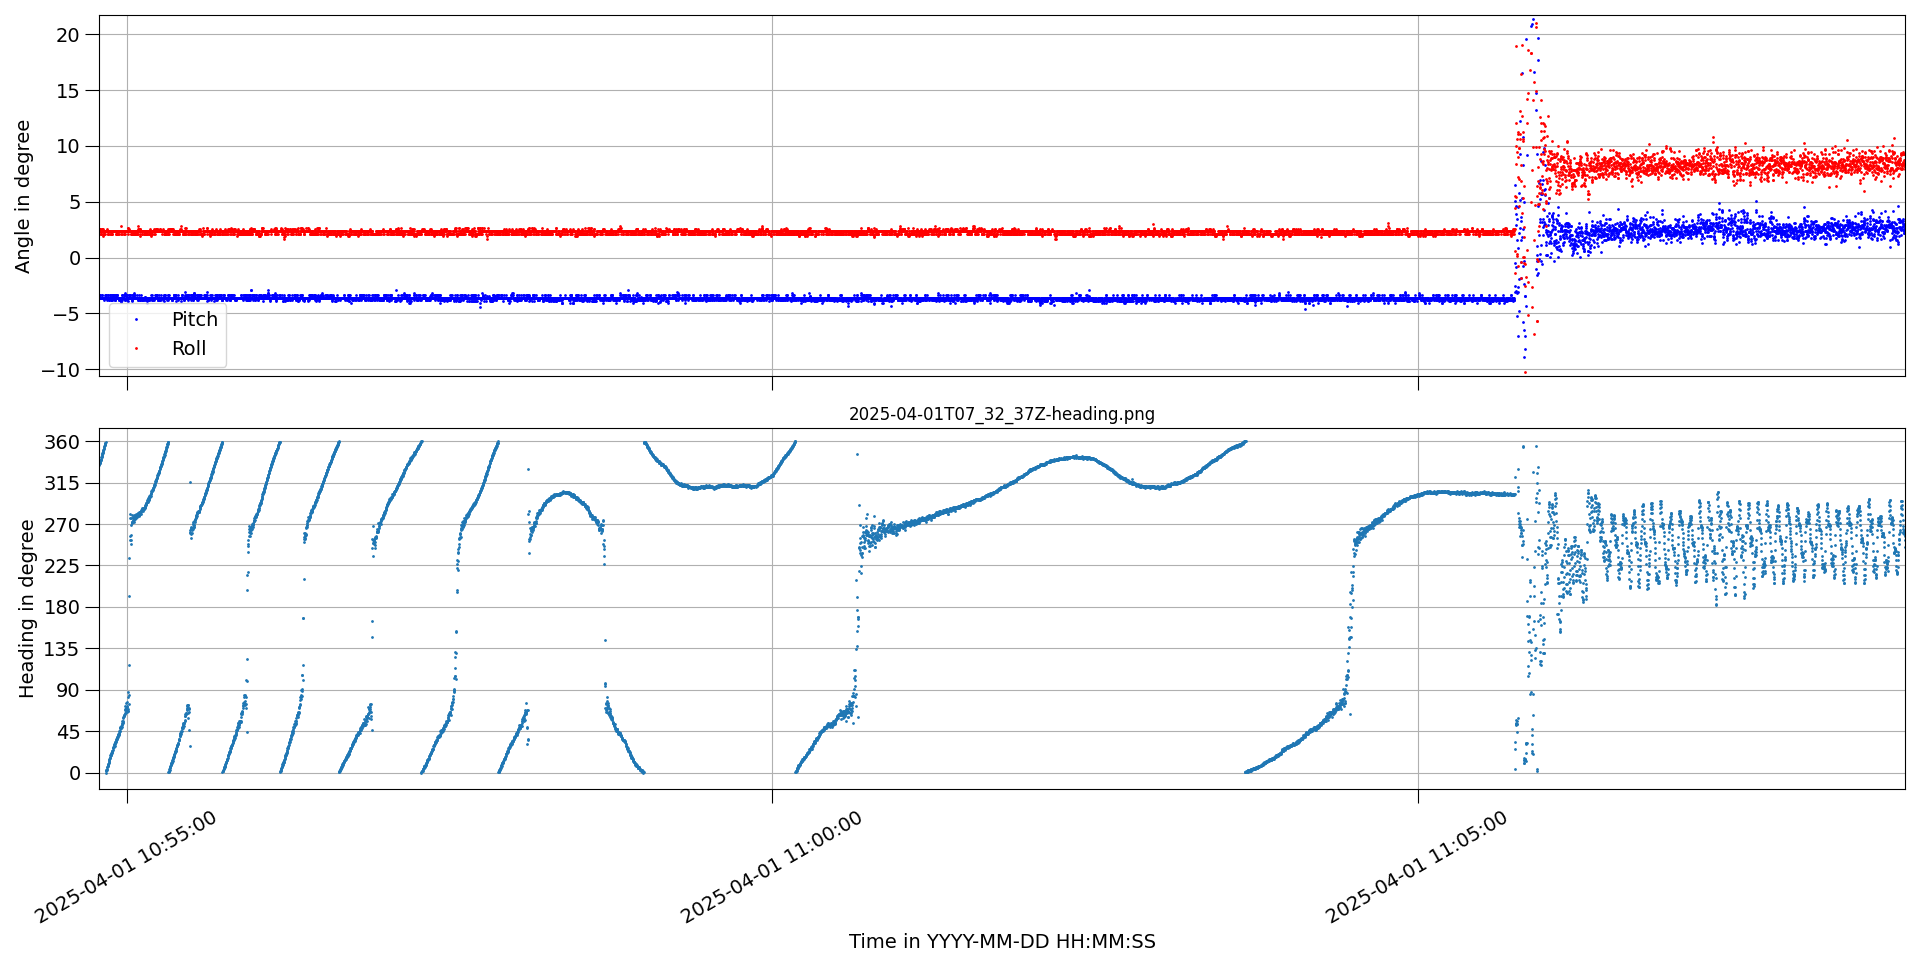
\includegraphics[width=\linewidth]{images/05_flight_data/pop_heading.png}
    \caption[Heading at balloon burst.]{Pitch, roll and heading balloon burst.}
    \label{fig:res:burst_heading}
\end{figure}


\section{Descent \label{sec:descent}}
The last flight phase is the descent of the payload. At this time, a parachute has opened up and is producing drag to slow the box to an equilibrium velocity. As can be seen in fig.~\ref{fig:res:descent_heading}, roll and pitch angles are offset by 5 and 10 degrees each. This may be again because the attachment of the parachute is not perfectly centred, and the centre of gravity is not on the vertical axis. Each angle has a peak-to-peak amplitude of approximately $5^\circ$.\\
In the lower plot in fig.~\ref{fig:res:descent_heading}, it can be seen that the gondola is not spinning after the burst. Sporadically, the box will perform a rotation, which gets more frequent until around 11:32~UTC when the gondola begins to spin with a frequency of approximately 5~rpm.

\begin{figure}[H]
    \centering
    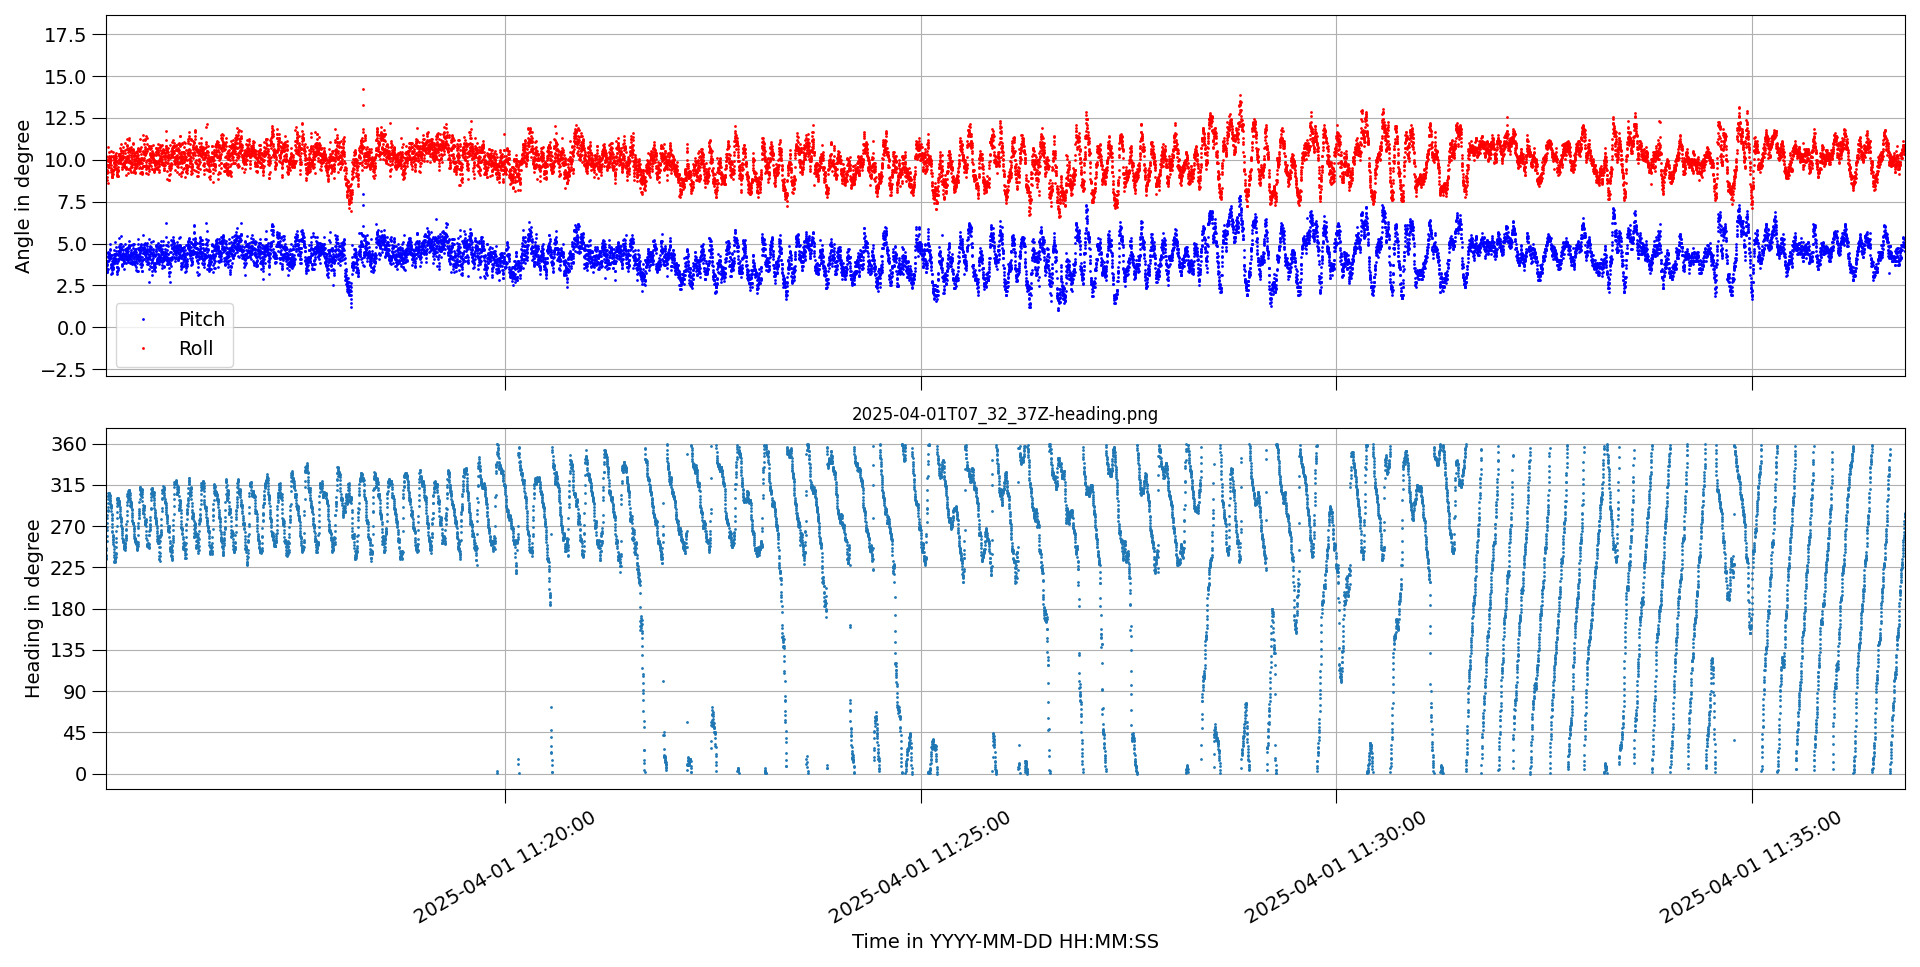
\includegraphics[width=\linewidth]{images/05_flight_data/descend_heading.png}
    \caption[Heading during descent.]{Pitch, roll and heading during descent.}
    \label{fig:res:descent_heading}
\end{figure}